\chapter{Tarea}
\justifying
\begin{enumerate}
    \item Resolver los siguientes problemas: 
    
    \textbf{15-b)} Resolver
    $$(3x+2y+y^2)dx+(x+4xy+5y^2)dy=0$$
    con el factor integrante $\mu = \varphi(x+y^2)$
    \begin{sol}
    Para que $\mu$ sea factor integrante, debe verificarse que
    $$\pd{\mu \: (3x+2y+y^2)}{y}=\pd{\mu \: (x+4xy+5y^2)}{x}$$
    y integrando por separado cada parte de la igualdad:
    $$\pd{\mu \: (3x+2y+y^2)}{y}=\pd{\varphi(x+y^2)\: 3x}{y}+ \pd{\varphi(x+y^2) \: 2y}{y}+\pd{\varphi(x+y^2) \: y^2}{y}=$$
    $$=\pd{\varphi(x+y^2)}{y}\: 3x +\cancel{\pd{3x}{y}}\varphi(x+y^2)+ \pd{\varphi(x+y^2)}{y} \: 2y + \pd{2y}{y} \varphi(x+y^2) + \pd{\varphi(x+y^2)}{y} \: y^2 + \pd{y^2}{y} \varphi(x+y^2) = $$
    $$= 6xy \:\varphi'(x+y^2) + 4y^2 \varphi'(x+y^2) + 2 \varphi(x+y^2) + 2y^3 \varphi'(x+y^2)+2y \varphi(x+y^2)=$$
    $$=(6xy+4y^2+2y^3)\mu'+(2+2y)\mu$$

    $$\pd{\mu \: (x+4xy+5y^2)}{x}=\pd{\varphi(x+y^2)\: x}{x}+\pd{\varphi(x+y^2)\: 4xy}{x}+\pd{\varphi(x+y^2)\: 5y^2}{x}=$$
    $$=x\pd{\varphi(x+y^2)}{x}+\cancel{\pd{x}{x}}\varphi(x+y^2) + \pd{\varphi(x+y^2)}{x} 4xy +\varphi(x+y^2) \pd{4xy}{x}+\pd{\varphi(x+y^2)}{x}5y^2+\cancelto{0}{\pd{5y^2}{x}\varphi(x+y^2)}=$$
    $$=x\mu'+\mu+4xy\mu'+4y\mu+5y^2\mu'=(x+4xy+5y^2)\mu'+(1+4y)\mu$$
    e igualando lo obtenido en ambas partes de la igualdad,
    $$(6xy+4y^2+2y^3)\mu'+(2+2y)\mu=(x+4xy+5y^2)\mu'+(1+4y)\mu \; \iff $$
    $$\; (6xy+4y^2+2y^3 - x-4xy-5y^2)\mu'=(1+4y-2-2y)\mu  \; \iff \; \mu'=\dfrac{-1+2y}{2xy-x-y^2+2y^3} \mu$$
    simplificando el cociente
    $$\dfrac{-1+2y}{2xy-x-y^2+2y^3}=\dfrac{2y-1}{x(2y-1)+y^2(-1+2y)}=\dfrac{\cancel{2y-1}}{\cancel{(2y-1)}(x-y^2)}=\dfrac{1}{x+y^2}$$
    luego 
    $$\varphi'(x+y^2)=\dfrac{\varphi(x+y^2)}{x+y^2} \; \overset{*}{\Rightarrow} \; \varphi(x+y^2)=k(x+y^2) \; \quad k \in \mathbb R$$
    $^*$ considerando $x+y^2=t$, la ecuación es $\varphi'(t)-\dfrac{1}{t}\varphi(t)=0$, entonces $\varphi(t)=k \: t=k (x+y^2)$
    así que la ecuación, ya exacta es 
    $$k (x+y^2)(3x+2y+y^2)dx+k (x+y^2)(x+4xy+5y^2)dy=0$$
    y resolverla es encontrar una función potencial $F$ (dado que es una, elegimos $k=1$) tal que $\omega=dF$, luego 
    $$\left\{ \begin{array}{l}
         \pd{F}{x}=A=(x+y^2)(3x+2y+y^2) \\
         \pd{F}{y}=B=(x+y^2)(x+4xy+5y^2) 
    \end{array}\right.$$
    luego por la primera ecuación,
    $$F(x,y)=\int (x+y^2)(3x+2y+y^2) dx=\int 3x^2+2xy+xy^2+3xy^2+2y^3+y^4 \: dx=$$
    $$=x^3+x^2y+2x^2y^2+2xy^3+xy^4+xy^5+\alpha(y)=x(x^2+xy+2xy^2+2y^3+y^4+y^5)+\alpha(y)$$
    y sutituyendo en la segunda ecuación del sistema anterior:
    $$\pd{}{y}\left(x(x^2+xy+2xy^2+2y^3+y^4+y^5)+\alpha(y)\right)=(x+y^2)(x+4xy+5y^2) $$
    luego, derivando respecto de $y$,
    $$\pd{}{y}(x^2+xy+2xy^2+2y^3+y^4+y^5)+\alpha(y))=x+4xy+6y^2+4y^3+5y^4+\alpha(y)'$$
    e igualando a $B$,
    $$x+4xy+6y^2+4y^3+5y^4+\alpha(y)'=x^2+4x^2y+5xy^2+xy^2+4xy^3+5y^4 \; \iff \; $$
    $$\alpha(y)' = 4 x^2 y + x^2 + 4 x y^3 + 6 x y^2 - 4 x y - x - 4 y^3 - 6 y^2 $$
    $$\alpha(y)=\int  4 x^2 y + x^2 + 4 x y^3 + 6 x y^2 - 4 x y - x - 4 y^3 - 6 y^2 dy =$$
    $$= 2 x^2 y^2 + x^2 y + x y^4 + 2 x y^3 - 2 x y^2 - x y - y^4 - 2 y^3 + c$$
    luego 
    $$F(x,y)=x^3+x^2y+2x^2y^2+2xy^3+xy^4+xy^5+2 x^2 y^2 + x^2 y + x y^4 + 2 x y^3 - 2 x y^2 - x y - y^4 - 2 y^3+c=$$
    $$x^3 + 4 x^2 y^2 + 2 x^2 y + x y^5 + 2 x y^4 + 4 x y^3 - 2 x y^2 - x y - y^4 - 2 y^3 + c $$
    \end{sol}
    \textbf{19.} Hallar la curva que pasa por el punto (1,1) para la cual la pendiente de la tangente
en cualquier punto es $n$ veces mayor que la pendiente de la recta que une dicho punto con el origen de coordenadas.
\begin{sol}
    Sea $y=f(x)$ la curva que queremos hallar, la pendiente de la recta que pasa por un punto $(x,f(x))$ y por $(0,0)$
    es $$m_1=\dfrac{f(x)-0}{x-0}=\dfrac{f(x)}{x}$$
    y por otro lado, la pendiente de la tangente en ese punto es 
    $$m_2=f'(x)$$
    y como pide el enunciado deben ser proporcionales, por lo que
    $$m_2=n\cdot m_1 \; \iff \; f'(x)=n \cdot \dfrac{f(x)}{x} \; \iff \; \dfrac{df(x)}{dx}=n \cdot \dfrac{f(x)}{x} \; \iff \; \dfrac{df(x)}{f(x)}=n \cdot \dfrac{dx}{x} \; \iff \; $$
    $$ \ln|f(x)|=n \cdot \ln|x| + C $$
    y como son las curvas que pasan por $(1,1)$, tenemos un problema de condiciones iniciales con $f(1)=1$, fijando la constante:
    $$\ln|f(1)|=n \cdot \ln|1|+C \; \iff \; C=0$$
    Entonces la ecuación de la curva es:
    $$\ln|f(x)|=n \cdot \ln|x|$$
Podemos escribir esto en forma exponencial:
$$|f(x)|=|x|^n$$
Si $x > 0$, entonces $f(x) = x^n$. Si $x < 0$, entonces $f(x) = -|x|^n$. En resumen, la curva que cumple las condiciones del problema está dada por la función:
$$f(x)=\left\{ \begin{array}{ll} x^n & \text{ si } x>0 \\ -|x|^n & \text{ si } x<0
\end{array}\right.$$
siendo $n$ una constante positiva. Veamos un ejemplo con $\textcolor{blue}{f(x)=x^3}$ en el que se represente:
$$\begin{tikzpicture}[scale=4, domain=1:-0.5, samples=50]
	
	% draw axis
	\draw[->] (-0.5,0) -- (1,0) node[below right] {$x$};
	\draw[->] (0,-0.2) -- (0,1) node[above left] {$y$};
	
	% draw function
	\draw[blue, thick] plot (\x, {\x*\x*\x}) node[left] {\footnotesize $f(x)$};
    \draw[red, thick,domain=0.5:1.1] plot (\x, {1.92*\x - 1.035}) node[right] {\footnotesize $f'(x)$};
    \def\x{0.8}
    \draw[fill=black] (\x,{\x*\x*\x}) circle [radius=0.01];
    \draw[orange,thick] (\x,{\x*\x*\x}) -- (0,0);	
\end{tikzpicture}$$
donde $\textcolor{orange}{m_1}=\nicefrac{f(0.8)}{0.8}=\nicefrac{0.512}{0.8}=\textcolor{orange}{0.64}$ y $\textcolor{red}{m_2}=f'(0.8)=3(0.8)^2=\textcolor{red}{1.92}$ y por tanto, $\textcolor{orange}{m_1}=3 \cdot \textcolor{red}{m_2}$.
\end{sol}
\textbf{23.}  La velocidad inicial de un barco es de 10 m/s; su movimiento se retrasa por la
acción de la resistencia del agua, que es proporcional a la velocidad del barco. Si a los 5 segundos su velocidad es de 8 m/s, ¿Después de cuánto tiempo la velocidad será de 1 m/s?
\begin{sol}
  La ecuación de movimiento será $F_{total}=ma$, y las fuerzas que actuan son la de resistencia y la que propulsa al barco, luego la ecuación final es
  $$F_{p}-kv=m\dfrac{dv}{dt} \: \iff \: \dfrac{dv}{dt}=\dfrac{F_p}{m}-\dfrac{k}{m}\: v \: \iff \: \dfrac{dv}{dt}=-\alpha \: v $$
  asumiendo una masa y una fuerza propulsora constante. De esta forma, integrando la ecuación, 
  $$v=C \: e^{-\alpha \: t}$$
  y las condiciones iniciales nos determinan las constantes, luego 
  $$v(0)=10=C \: e^0 \; \Rightarrow \; C=10 \qquad v(5)=10 \: e^{-5 \:\alpha }=8 \; \iff \; \alpha=\nicefrac{1}{5} \ln(\nicefrac{10}{8}) \approx 0.08664$$
  y la ecuación general es 
  $$v(t)=10 \: e^{-0.08664 \: t}$$
  luego para hallar el tiempo en el que $v=1$m/s,
  $$10 \: e^{-0.08664 \: t} = 1 \; \iff \; t=-\dfrac{1}{0.08664}\ln(\nicefrac{1}{10}) \approx 11.54 s$$
\end{sol}

\textbf{25-h)} $x=y'+\sin(y')$
\begin{sol}
    Llamando $p=y'$ y por la regla de la cadena:
    $$\dfrac{dy}{dx}=\dfrac{\nicefrac{dy}{dp}}{\nicefrac{dx}{dp}}$$
    donde 
    $$\dfrac{dx}{dp}=\dfrac{d}{dp} (p + \sin (p))=1+\cos(p) \qquad \dfrac{dy}{dx}=p$$
    luego, por la regla de la cadena
    $$ \dfrac{dx}{dp} \cdot \dfrac{dy}{dx}=\dfrac{dy}{dp} \; \iff \; (1+\cos(p)) p = \dfrac{dy}{dp} \; \iff \; y=\int p + p \cos(p) \: dp=$$
    $$=\int p \:  dp + \int p \cdot \cos (p) \: dp = \dfrac{p^2}{2}+ p \sin (p) - \int \sin (p) \: dp=\dfrac{p^2}{2}+ p \cdot \sin (p) + \cos(p)$$
    Es decir, las variables $x$ e $y$ quedan parametrizadas respecto de $p$ como
    $$\boxed{ \; x=p+\sin(p) \qquad y=\dfrac{p^2}{2}+ p \cdot \sin (p) + \cos(p) + k \;} \qquad k \in \mathbb R$$
    y el Teorema de las Funciones Implícitas asegurará o no la posibilidad de despejar $y$ en función de $x$.
\end{sol}
\textbf{33.}  Introduciendo una nueva incógnita, integrar el sistema siguiente reduciéndolo a
uno de primer orden:
$$\left\{\begin{array}{l} x''=-11x+4y \\ y'=-15x+6y\end{array}\right.$$
\begin{sol}
    Sea $x'=p$, podemos reescribir el sistema como
    $$\left\{ \begin{array}{l}
         x'' = -11x + 4y  \\
         y' = -15x + 6y
    \end{array}\right. \iff \left\{ \begin{array}{l}
         x' = p \\
         p' = -11x+4y\\
         y' = -15x + 6y
    \end{array}\right. \longleadsto{0.5} \begin{pmatrix}
        x' \\ p' \\ y'
    \end{pmatrix}=\begin{pmatrix}
        0 & 1 & 0 \\
        -11 & 0 & 4 \\
        -15 & 0 & 6
    \end{pmatrix} \begin{pmatrix}
        x \\ p \\ y 
    \end{pmatrix}$$ 
    de forma que, denotando
    $$A=\begin{pmatrix}
        0 & 1 & 0 \\
        -11 & 0 & 4 \\
        -15 & 0 & 6
    \end{pmatrix}$$
    la solución al sistema es $Y=e^{tA} C$ donde la descomposición de Jordan de la matriz es $A=B J B^{-1}$, luego para hallarla, calculamos el polinomio característico
    $$c_A(x)=|x \: Id- A|=\begin{vmatrix}
        x & -1 & 0 \\
        11 & x & -4 \\
        15 & 0 & x-6
    \end{vmatrix}=x^2(x-6)+60+11(x-6)=x^3-6x^2+11x-6$$
    $$=(x-1)(x-2)(x-3)$$
    y por tanto, la matriz diagonaliza como
    $$J=\begin{pmatrix}
        1 & 0 & 0 \\
        0 & 2 & 0 \\
        0 & 0 & 3
    \end{pmatrix}$$
    y por tanto la solución es $Y=B e^{tD} B^{-1} C$ siendo $B$ la matriz del cambio de base de $A$ a $J$, dada por la base de vectores propios $\{e_1, e_2, e_3\}$ (donde $e_i \in \ker(T-\lambda_i Id)$ siendo $\lambda_i$ los valores propios). Calculando dichos vectores propios
    $$\ker (T-Id) \equiv \begin{pmatrix}
        0 & 0 & 0 \\
        0 & 1 & 0 \\
        0 & 0 & 2
    \end{pmatrix}\begin{pmatrix}
        x \\ y \\ z
    \end{pmatrix}=\begin{pmatrix}
        0 \\ 0 \\ 0
    \end{pmatrix} \equiv \left\{ \begin{array}{l}
         y=0  \\
          2z=0
    \end{array} \right. \equiv \left\{ \begin{array}{l}
         y=0  \\
         z=0
    \end{array} \right.  \equiv <(x,0,0)>$$
    $$\ker (T-2Id) \equiv\begin{pmatrix}
        -1 & 0 & 0 \\
        0 & 0 & 0 \\
        0 & 0 & 1
    \end{pmatrix} \begin{pmatrix}
        x \\ y \\ z
    \end{pmatrix}=\begin{pmatrix}
        0 \\ 0 \\ 0
    \end{pmatrix}\equiv \left\{ \begin{array}{l}
         -x=0  \\
          -z=0
    \end{array} \right.\equiv \left\{ \begin{array}{l}
         x=0  \\
        z=0
    \end{array} \right. \equiv  <(0,y,0)>$$
    $$\ker (T-3Id) \equiv \begin{pmatrix}
        -2 & 0 & 0 \\
        0 & -1 & 0 \\
        0 & 0 & 0
    \end{pmatrix}\begin{pmatrix}
        x \\ y \\ z
    \end{pmatrix}=\begin{pmatrix}
        0 \\ 0 \\ 0
    \end{pmatrix} \equiv \left\{ \begin{array}{l}
         -2x=0  \\
          -y=0
    \end{array} \right. \equiv \left\{ \begin{array}{l}
         x=0  \\
         y=0
    \end{array} \right. \equiv <(0,0,z)> $$
    luego una base es $\{(1,0,0),(0,1,0),(0,0,1)\}$ y por tanto la matriz del cambio de base $B=Id$. De esta forma
    $$Y=B e^{tD} B^{-1} C=e^{tD} C=\begin{pmatrix}
        e^t & 0 & 0 \\
        0 & e^{2t} & 0 \\
        0 & 0 & e^{3t}
    \end{pmatrix} \begin{pmatrix}
        c_1 \\ c_2 \\ c_3
    \end{pmatrix}=  \begin{pmatrix}
        c_1 \: e^{t}  \\ c_2 \: e^{2t} \\ c_3 \: e^{3t} 
    \end{pmatrix} =\begin{pmatrix}
        x \\ p \\ y 
    \end{pmatrix}$$
    Es decir, las soluciones del sistema son 
    $$x=c_1 \: e^{t}  \qquad   p = x' = c_2 \: e^{2t} \qquad y = c_3 \: e^{3t} $$
    y dado que tenemos una solución para $x'$, integrando
    $$x'=\dfrac{dx}{dt}=c_2 \: e^{2t} \; \iff \; x=\dfrac{c_2}{2} e^{2t}$$
    y por tanto, 
    $$x=c_1 \: e^{t} + k_2 \: e^{2t}$$
\end{sol}
\textbf{43-e)}$(1+x^2)y''+(y')^2+1=0$
\begin{sol}
    Sea $y'=p$, entonces
    $$p'(1+x^2)+p^2+1=0 \; \iff \; \dfrac{dp}{dx}=\dfrac{-1-p^2}{1+x^2} \; \iff \; \dfrac{dp}{-1-p^2}-\dfrac{dx}{1+x^2}=0 \; \iff $$
    $$\iff \; d\left(\int \dfrac{dp}{-1-p^2} - \int \dfrac{dx}{1+x^2} \right)=0 \; \iff \; \int \dfrac{dp}{-1-p^2} - \int \dfrac{dx}{1+x^2} = c \; \iff $$
    $$ \iff \; -\arctan(p)-\arctan(x)=c \; \iff \; p=-\tan (c+\arctan(x))$$
    y deshaciendo el cambio de variable $p=y'$
    $$\dfrac{dy}{dx}=-\tan (c+\arctan(x)) \; \iff \; y=\int -\tan (c+\arctan(x)) dx$$
    y usando la fórmula de la tangente de la suma $\left(\tan(a+b)=\frac{\tan(a)+\tan(b)}{1-\tan(a)\tan(b)}\right)$,
    $$y=\int -\tan (c+\arctan(x)) dx=-\int \dfrac{k+x}{1-kx} \: dx = \int \dfrac{-k}{1-kx} \: dx  - \int \dfrac{x}{1-kx} \: dx = $$
    $$=\log|1-kx| + x \dfrac{\log|1-kx|}{k} - \int \dfrac{\log|1-kx|}{k} dx =$$
    $$=\log|1-kx| + x \dfrac{\log|1-kx|}{k} - \dfrac{( k x-1 ) \log|1 - k x| - kx}{k^2} = \dfrac{k x + (1 + k^2) \log|1 - k x|}{k^2} $$  
\end{sol}

\textbf{46-b)} Resolver la ecuación de Euler:
$$x^2y''-xy'+2y=x \: \log(x)$$
\begin{sol}
    Haciendo el cambio de variable $x=e^t$, e $y'=\nicefrac{dy}{dx}$ e $\dot{y}=\nicefrac{dy}{dt}$, por la regla de la cadena $y'=\nicefrac{\dot{y}}{x}$ y de la misma forma, $y''=\nicefrac{\ddot{y}-\dot{y}}{x^2}$ luego
    $$x^2y''-xy'+2y=x \: \log(x) \; \equiv \; \ddot{y}-\dot{y}-\dot{y}+2y=e^t \: t \; \equiv \; (D^2-2D+2)y=t \: e^t$$
    Completando el cuadrado, $D^2-2D+2=D^2-2D+1+1=(D-1)^2+1^2$, luego las \underline{soluciones homogéneas} vienen dadas por 
    $$\ker((D-1)^2+1^2)=<e^{-t} \: \sin(t), e^{-t} \: \cos (t)>$$
    luego denotaremos  $y_h=c_1 \: e^{-t} \: \sin(t) + c_2 \: e^{-t} \: \cos (t)$
    
    Por otro lado, para hallar una \underline{solución particular} invertimos el operador, y dado que $D^2-2D+2=(D-(1+i))(D-(1-i))$, entonces
    $$(D-(1+i))(D-(1-i))y=b(t) \; \iff \; y = \dfrac{1}{D-(1+i)} \cdot \dfrac{1}{D-(1-i)} b(t)$$
    Pudiendo separar ambos operadores. En primer lugar
    $$\dfrac{1}{D-(1-i)} b(t)=e^{-(1-i)t}e^{(1-i)t}\dfrac{1}{D-(1-i)} b(t)=e^{(1-i)t}\dfrac{1}{D} e^{-(1-i)t} b(t)=e^{(1-i)t} \int e^{-(1-i)t} b(t) \: dt $$
    y de la misma forma:
    $$y_p=\dfrac{1}{D-(1+i)} \cdot \dfrac{1}{D-(1-i)} \: b(t)=\dfrac{1}{D-(1+i)} \: e^{(1-i)t} \int e^{-(1-i)t} b(t) \: dt = $$
    $$=e^{(1+i)t} e^{-(1+i)t}\dfrac{1}{D-(1+i)} \: e^{(1-i)t} \int e^{-(1-i)t} b(t) \: dt =e^{(1+i)t} \dfrac{1}{D} e^{-(1+i)t} \: e^{(1-i)t} \int e^{-(1-i)t} b(t) \: dt =$$
    $$=e^{(1+i)t} \int \left( e^{-2it} \int e^{-(1-i)t} e^t \: t \: dt \right) \:dt=e^{(1+i)t} \int \left( e^{-2it} \int e^{it} \: t \: dt \right) \:dt=$$
    $$=e^{(1+i)t} \int \left( e^{-2it} e^{it} (1-it)\right) \:dt =e^{(1+i)t} \int  e^{-it} (1-it)\: dt =e^{(1+i)t} e^{-it} t =e^t \: t $$
\end{sol} 
y la solución general es 
$$y=y_p+y_h= t e^t \: e^{-t} \: \sin(t) + t e^t e^{-t} \: \cos (t) + k \: e^t \: t $$
y deshaciendo el cambio de variable 
$$y= \log|x| \: \sin(\log(x)) + \log|x| \: \cos (\log(x)) + k x \: \log (x)$$
\item Fijemos dos puntos del plano $F_1$ y $F_2$. Se sabe que cada curva elíptica $E$ con focos $F_1$ y $F_2$ cumple la siguiente propiedad: un rayo de luz que parte de $F_1$ y se refleja en esa curva, pasará después por $F_2$. Se pide demostrar que sólo esas elipses (o arcos de ellas) satisfacen
dicha propiedad.
\begin{sol}
    Véase la figura
    $$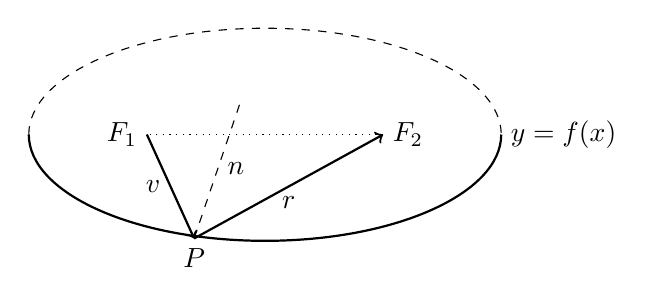
\begin{tikzpicture}[scale=1.5]
  \coordinate [label=left:$F_1$] (F1) at (0,0);
  \coordinate [label=right:$F_2$] (F2) at (2,0);
  \draw [dotted] (F1) -- (0,0);
  \draw [dotted] (F2) -- (0,0);
  \draw [thick] (-1,0) arc (180:360:2 and 0.9);
  \draw [dashed] (-1,0) arc (180:0:2 and 0.9) node [right] {$y=f(x)$} ;
  \coordinate [label=below:$P$] (P) at (0.4,-0.88);
  \draw [thick,->] (F1) -- (P) node [midway,left] {$v$} ;
  \draw [thick,->] (P) --  (F2) node [midway,below] {$r$};
  \draw [dashed] (P) -- (0.8,0.3) node [midway,right] {$n$};
\end{tikzpicture}$$
 de forma que $v$ es la recta del rayo que parte de $F_1$ y $r$ la recta del ángulo reflejado, y que por tanto, al tratarse de una reflexión, se debe verificar que $$\widehat{(v,n)}=\widehat{(n,r)}=\theta$$
 Los vectores directores de cada recta son, considerando $F_1=(-c,0)$, $F_2=(c,0)$ y $P=(x_o,y_o)$ 
 $$u_v=(x_o-c,y_o) \qquad u_n=(y'(x_o), -1) \qquad u_r=(c-x_o,-y_o)$$
 por tanto
 $$\cos \theta=\dfrac{u_v \cdot u_n}{|u_v|\cdot \cancel{|u_n|}}=\dfrac{u_r \cdot u_n}{|u_r|\cdot \cancel{|u_n|}} $$
 $$\iff \dfrac{(x_o-c)y'_o-y_o}{\sqrt{(x_o-c)^2+y_o^2}}=\dfrac{(c-x_o)y'_o+y_o}{\sqrt{(c-x_o)^2+y_o^2}}\iff $$
 $$\iff \left((x_o-c)y'_o-y_o\right) \sqrt{(c-x_o)^2+y_o^2} - \left((c-x_o\right)y'_o+y_o) \sqrt{(x_o-c)^2+y_o^2} = 0$$
 Dado que queremos que se verifique para todo $x_o,y_o$, obviamos los subíndices y la ecuación implícita final es
 $$\left((x-c)y'-y\right) \sqrt{(c-x)^2+y^2} - \left((c-x\right)y'+y) \sqrt{(x-c)^2+y^2} = 0$$
 y simplificadamente (detalles al final):
 $$2((x-c)y'-y) \sqrt{(x-c)^2 + y^2}= 0 $$
Despejamos $y'$, y reordenamos los términos de forma que obtenemos la ecuación
$$y'-\dfrac{1}{2x-2c}y=0 \; \iff \; y=k\sqrt{c-x}$$ \textcolor{red}{waaaaaa :( }
 
 
 para comprobar la unicidad de soluciones, usaremos el Teorema para Funciones Implícitas, que enuncia que \vspace{5mm}

 Si $F \in \mc{C}^1$ y $q_o = (x_o,y_o,y_o') $ tal que $$F(q_o)=0 \qquad \text{ y } \qquad \left( \pd{F}{p} \right)_{q_o} \neq 0$$ entonces el problema de valores iniciales
 $$\left\{ \begin{array}{l}
      F(x,y,y')= 0 \\ y(x_o)=y_o \\ y'(x_o)=p_o
 \end{array} \right.$$
 tiene una solución $y(x)$ en un intervalo de $x_o$ y en ese intervalo es única.

 Entonces
 $$\pd{F}{p}= \pd{}{p} \: \left(2((x-c)y'-y) \sqrt{(x-c)^2 + y^2} \right) = 2(x-c)\sqrt{(x-c)^2+y^2} $$
 y por tanto, 
 $$\left( \pd{F}{p} \right)_{q_o} =   2(x_o-c)\sqrt{(x_o-c)^2+y_o^2}\neq 0 \; \iff \; x_o \neq c$$
 luego existen soluciones y son únicas.

La simplificación de la ecuación se hace como sigue:
Observemos que $(c-x)^2=(x-c)^2$ ambas expresiones son iguales, por lo tanto, podemos reemplazar una por la otra y simplificar la expresión dada:
\begin{align*}
&\left((x-c)y'-y\right) \sqrt{(c-x)^2+y^2} - \left((c-x)y'+y\right) \sqrt{(x-c)^2+y^2}\\
&= \left((x-c)y'-y\right) \sqrt{x^2 - 2cx + c^2 + y^2} - \left((c-x)y'+y\right) \sqrt{x^2 - 2cx + c^2 + y^2}\\
&= \left((x-c)y' - y - (c-x)y' - y\right) \sqrt{x^2 - 2cx + c^2 + y^2}\\
&= 2((x-c)y'-y)  \sqrt{(x-c)^2 + y^2}
\end{align*}
Por lo tanto, la expresión simplificada es $2((x-c)y'-y) \sqrt{(x-c)^2 + y^2}$.
\end{sol}

\item \justifying  Partiendo del método de variación de las constantes para sistemas de ecuaciones lineales de primer orden, obtener ($=$ enunciar y demostrar) ese mismo método en el caso de una ecuación lineal de orden superior. Ilustrarlo con un ejemplo de segundo orden. \footnote{L. Esgoltz: \textit{Ecuaciones diferenciales y cálculo variacional}. 1969, pp. 119-122.}
\begin{sol}
Está en los métodos de resolución.
\end{sol}

\item \justifying Sea $f : \mathbb R^n \longrightarrow \mathbb R^n$ una aplicación de clase $\mc{C}^1$ y sea $Y_o$ un punto de $\mathbb R^n$. Supongamos que la imagen de toda solución del problema de
condiciones iniciales $Y' = f(Y ), \: Y (0) = Y_o$ permanece en un cierto compacto $K \subset \mathbb R^n$. Probar que existe una solución ``global'' a ese problema, es decir, una solución $Y = Y (t)$ definida para todo $t \in \mathbb R$.
\begin{sol}
    Dado que $f$ es de clase $\mc{C}^1$, es diferenciable, y sea su derivada $d_pf$, en un entorno $U \ni p$ la derivada está acotada (por ser continua), de forma que por el Teorema de Valor Medio, 
    $$\|f(y)-f(x)\|\leq \| d_pf \|\cdot  \|y-x\|$$
    donde $p \in I[x,y] \subset U$ es el segmento que une $x$ e $y$. 

    De esta forma, podemos asegurarnos que $f$ es localmente de Lipschitz en $U$ ya que 
    $$\|f(y)-f(x)\|\leq L \cdot   \|y-x\|$$
    eligiendo $\displaystyle L=\sup_{p \in U} \|d_pf\|$ el cual existe por estar acotada, como hemos mencionado. Aseguramos así la existencia de soluciones por el Teorema de Existencia y Unicidad para sistemas de ecuaciones lineales en $U$. Para extender la solución a $\mathbb R$, basta saber que en un compacto, toda función continua alcanza su máximo y su mínimo de forma que, por $f \in \mc{C}^1$, $d_pf$ es continua ($\forall p$) y por tanto se verifica la condición de Lipchitz en todo $K \subset \mathbb R^n$. 

    Y por último, hemos visto que se verifica la condición de Lipchitz para segmentos del tipo $[x,y]=[t_o-\alpha,t_o+\alpha]$, (siendo $t_o$ el punto medio), en dichos intervalos las soluciones $Y(t)$ son únicas, y de la misma forma que para el caso de una variable, podemos extender $I$ a $\mathbb R$ por ser $f$ contractiva en $K$, que es donde se encuentran las soluciones del problema de Cauchy.  
\end{sol}
\end{enumerate}